\documentclass[11pt,a4paper]{article}
\usepackage{fontspec}
\setmainfont{NotoSerifCJKkr-Regular.otf}[Path=fonts/,BoldFont=NotoSerifCJKkr-Bold.otf,ItalicFont=NotoSerifCJKkr-Regular.otf]
\setsansfont{NotoSerifCJKkr-Regular.otf}[Path=fonts/,BoldFont=NotoSerifCJKkr-Bold.otf]
\setmonofont{DejaVu Sans Mono}[Scale=0.79]
\XeTeXlinebreaklocale "ko"
\XeTeXlinebreakskip=0pt plus 1pt
\usepackage[margin=23mm,top=23mm,bottom=23mm,headheight=15pt]{geometry}
\usepackage{amsmath,amssymb,amsthm,mathtools,mathrsfs}
\usepackage{booktabs,tabularx,longtable,array,graphicx,float}
\usepackage[dvipsnames]{xcolor}
\usepackage{enumitem,caption,fancyhdr,titlesec}
\usepackage{tikz}
\usetikzlibrary{arrows.meta,positioning,calc}
\usepackage{hyperref}
\providecommand{\tightlist}{\setlength{\itemsep}{0pt}\setlength{\parskip}{0pt}}
\newcommand{\passthrough}[1]{#1}
\hypersetup{unicode=true,colorlinks=true,linkcolor=MidnightBlue,urlcolor=MidnightBlue,citecolor=MidnightBlue,pdftitle={WU088 HH PHYS19: HH와 birth의 순수 곡률과 검증된 유한 응답},pdfauthor={WU088 HH 연구}}
\urlstyle{same}
\setlength{\emergencystretch}{3em}
\setlength{\parskip}{0.34em}
\setlength{\parindent}{1em}
\widowpenalty=10000\clubpenalty=10000
\linespread{1.10}
\setlist{itemsep=0.18em,topsep=0.35em,leftmargin=1.6em}
\captionsetup{font=small,labelfont=bf}
\renewcommand{\figurename}{그림}
\renewcommand{\tablename}{표}
\renewcommand{\contentsname}{목차}
\renewcommand{\refname}{참고 문헌과 원자료}
\renewcommand{\proofname}{증명}
\titleformat{\section}{\large\sffamily\bfseries\color{MidnightBlue}}{\thesection}{0.7em}{}
\titleformat{\subsection}{\sffamily\bfseries}{\thesubsection}{0.7em}{}
\pagestyle{fancy}\fancyhf{}
\fancyhead[L]{\small\sffamily WU088\_HH / PHYS19 이론}
\fancyhead[R]{\small\sffamily 2026-10-13 UTC}
\fancyfoot[C]{\thepage}
\newcommand{\dd}{\mathrm d}
\newcommand{\diag}{\operatorname{diag}}
\newcommand{\ex}{\operatorname{exact64}}
\newcommand{\BB}{\mathcal B}
\newcommand{\HF}{\mathcal H_F}
\newcommand{\R}{\mathsf R}
\newcommand{\RF}{\mathsf R_F}
\newcommand{\ew}{e_w}
\newcommand{\exx}{e_x}
\newcommand{\nS}[1]{\left\lVert#1\right\rVert_S}
\newcommand{\nI}[1]{\left\lVert#1\right\rVert_\infty}
\newcommand{\magv}{\operatorname{mag}}
\newtheorem{theorem}{정리}
\newtheorem{lemma}{보조정리}
\newtheorem{proposition}{명제}
\theoremstyle{definition}\newtheorem{definition}{정의}

\begin{document}
\begin{titlepage}
\vspace*{14mm}
{\sffamily\bfseries\color{MidnightBlue}\Large WU088\_HH / PHYS19\par}
\vspace{8mm}
{\huge\bfseries HH와 birth의 순수 곡률과\\[3mm]검증된 유한 응답\par}
\vspace{7mm}
{\large 같은 gas--photon 계열의 두 half-step 대 Full-step 온도 결함\par}
\vspace{10mm}
{\large 이론 연구 루프 · 2026년 10월 13일 UTC\par}
\vspace{12mm}
\noindent\textbf{이번 결과.}
PHYS18에서 확립한 동일 계열의 혼합 응답에 두 순수 2차 응답을 결합했다.
원 gas Hessian, 35개 photon slot, 단계별 carry와 검증된 Full 역연산자로
전체 $(\lambda,b)\in[0,1]^2$에서
\[
F_{\lambda\lambda}\in[-4.510292217171,-3.084478303660]10^{-14}\ {\rm K},
\]
\[
F_{bb}\in[-4.912098573204,-4.450662359403]10^{-11}\ {\rm K}
\]
를 얻었다. 여기서 $F=T_{\rm two\ half}-T_{\rm Full}$이다.
두 축에서 각각 엄격한 오목성이 성립하며, 혼합 응답을 함께 쓰면
Hessian은 전체 사각형에서 양·음 고유값을 하나씩 가진다.

\vspace{4mm}
\noindent 같은 계열의 네 corner로 만든 bilinear 보간 오차는
$6.145761081776\times10^{-12}\ {\rm K}$ 이하이고,
순수 곡률 중심 보정으로
$2.892887673208\times10^{-13}\ {\rm K}$ 이하가 된다.
이는 곡률에 의한 형상 재구성 오차다. 현재 계수 포함을 수치 중심값으로
바꾼 모델의 전체 오차 예산은 본문에서 따로 계산한다.

\vfill
\noindent\small
워크플로: physmath-research-loop 1.0.0, R1--R10 및 한정된 C1--C10 계산.
SciSpace·Exa 원전 대조, 실제 Wolfram 15.0.1·xAct 1.3.0 검산,
외향 구간 계산과 독립 검토를 결합했다.
원 실행 기록·정확한 유리수 endpoint·소스·인계 계약은 함께 제공한 연구 묶음에 있다.
\end{titlepage}

\tableofcontents
\newpage
\section{질문, 범위와 계산 결과}
\subsection{고정한 물리 계열}
이번 질문은 HH source 강도 $\lambda$와 photon birth 진폭 $b$가
한 구간의 온도 결함 $F$를 각각 얼마나 휘게 만드는가이다.
PHYS18의 허용 계수 선택 $\alpha$ 하나를 고정하고,
같은 COMMON과 모든 단계에 공통인 $(\lambda,b)\in[0,1]^2$를 사용했다.
각 $\alpha$의 실제 계열에 대해 도함수를 취하고, 포함은 그 허용 계열 전체에 균일하다.
원 source에 맞춘 geometric-isotropic $C^2$ closure, gas 영역과 연결 선분,
양의 분모 및 검증된 implicit root branch를 그대로 사용한다.
경계 도함수에는 계약의 열린 근방을 사용한다.

상태와 시간 길이는
\[
g=(x_{\rm HII},y_{\rm HeII},y_{\rm HeIII},w_{\rm eV/H}),\qquad
h=625000000\ {\rm s},\quad \Delta t_F=2h
\]
이며, $t_0=160000000000\ {\rm s}$,
$t_1=160625000000\ {\rm s}$,
$t_2=161250000000\ {\rm s}$이다.
33개 활성 photon node와 number·energy guard 두 개를 모두 보존했다.
원 native leaves의 $c,\chi_H,k_B,\epsilon_{\rm eV}$를 사용하며,
밀도비는 저장된 두 밀도의 정확한 비
$f=\operatorname{exact}(n_{\rm He})/\operatorname{exact}(n_H)$다.
이 축소 source 계산에서 새 spacetime metric convention을 도입하지 않는다.

이 보고서에서 $F$와 그 매개변수 응답은 \emph{정의된 두 이산 경로 사이의 차이}다.
그 차이를 동일 물리 계열에서 정량적으로 해석하는 것이 이번 성과이며,
다음 소비 구간 연구에서는 원 HH source의 절대 열·전자 생성률을 별도로 읽는다.

\subsection{최종 외향 포함}
표의 decimal endpoint는 정확한 유리수 구간을 바깥 방향으로 표시했다.
혼합 응답과 첫 도함수는 PHYS17--18의 검증된 입력이고,
두 순수 도함수는 이번 실제 계산 결과다.
\begin{table}[H]\centering\small
\caption{같은 매개변수 사각형에서의 온도 응답. $\lambda,b$는 무차원이다.}
\begin{tabular}{lll}
\toprule
양 & Kelvin 단위 포함 & 근거\\
\midrule
$F_\lambda$ & $[-1.009599125635,-0.8137506081166]10^{-8}$ & 재사용\\
$F_b$ & $[6.776348385589,7.185335549648]10^{-5}$ & 재사용\\
$F_{\lambda b}$ & $[-2.668505746423,-2.118796636045]10^{-12}$ & PHYS18\\
$F_{\lambda\lambda}$ & $[-4.510292217171,-3.084478303660]10^{-14}$ & PHYS19\\
$F_{bb}$ & $[-4.912098573204,-4.450662359403]10^{-11}$ & PHYS19\\
\bottomrule
\end{tabular}
\end{table}

따라서 $\lambda$를 증가시키면 $F$는 감소하고 그 기울기는 더 음수가 된다.
$b$를 증가시키면 $F$는 증가하되 그 증가율은 줄어든다.
두 진술은 같은 사각형 위의 엄격한 축별 오목성과 함께 성립한다.
PHYS18의 $F_{\lambda b}<0$는 다른 축을 늘렸을 때 해당 기울기가
낮아지는 교차 응답을 제공한다.

\subsection{상관된 식으로 확보한 부호}
동일한 $K_d=g_{2,\theta\theta}-g_{F,\theta\theta}$에 대한 직접식과
상관식, 별도 endpoint 차이, 온도 차이를 교차했다.
직접식만으로 얻은 $\lambda$ 곡률은
$[-1.637584401887,1.098225441163]10^{-13}\ {\rm K}$로 0을 포함한다.
작은 $d,d_\theta,s,s_\theta$를 먼저 묶은 식은 표의 음의 포함을 닫는다.
$b$에서도 직접식의
$[-5.561103552739,-3.810012772503]10^{-11}\ {\rm K}$가 최종 구간으로 줄어든다.
이는 같은 방정식의 상쇄 구조를 보존해서 얻은 포함 개선이다.

\subsection{어떤 항이 순수 곡률을 만드는가}
각 residual sector를 같은 Full inverse와 온도 covector로 전달했다.
sector 사이의 상관은 원 계열에 남으므로 아래 항목은 그 공통 분해에서의 포함이다.
독립적으로 조정 가능한 물리 source로 해석하지 않는다.
\begin{table}[H]\centering\small
\caption{주요 부호 기여. 모든 수치는 K이다.}
\begin{tabularx}{\textwidth}{lXl}
\toprule
응답 & 항의 의미 & 온도 기여 포함\\
\midrule
$\lambda\lambda$ & HH gradient와 단계 tangent 증가분 &
$[-4.521186330242,-3.110103255620]10^{-14}$\\
$bb$ & 두 단계 opacity 변화 &
$[-1.041112989844,-0.9820550711823]10^{-11}$\\
$bb$ & birth의 backward-Euler 항 &
$[-1.638994735688,-1.387256337694]10^{-11}$\\
$bb$ & endpoint birth gradient와 tangent 결함 &
$[-2.074669289761,-1.956181232491]10^{-11}$\\
\bottomrule
\end{tabularx}
\end{table}

첫 행의 정확한 gas forcing은 $-2hDq_2[s_\lambda]\nu_H$이다.
그 포함폭 $1.411083074621\times10^{-14}\ {\rm K}$가
$\lambda$ 곡률 포함폭의 대부분을 차지한다.
$b$에서는 birth와 상태 의존 생존확률의 곱,
stage opacity 차이, endpoint의 같은 birth 응답이 함께 지배한다.
순수 곡률이 작은 이유와 부호를 이 실제 항들에 연결할 수 있다.

\section{전체 Hessian의 방향 구조}
\[
\nabla^2 F=
\begin{pmatrix}A&M\\M&D\end{pmatrix},
\qquad A=F_{\lambda\lambda},\quad M=F_{\lambda b},\quad D=F_{bb}.
\]
세 포함을 정확한 유리수 interval 연산으로 결합하면
\[
\det\nabla^2F\in[-5.748125770240,-2.273799188447]10^{-24}\ {\rm K}^2<0.
\]
그러므로 각 매개변수 점에서 Hessian은 양·음 고유값을 하나씩 가진다.
이를 고정 방향으로도 구성할 수 있다:
\[
v=(1,-1/24),\qquad
v^T\nabla^2Fv=A-\frac{M}{12}+\frac{D}{576}
\in[4.618397504729,11.42622520923]10^{-14}\ {\rm K}>0.
\]
$w=(1,0)$에서는 $w^T\nabla^2Fw=A<0$이다.
따라서 $[0,1]^2$ 안에 놓인 $v$ 방향 선분의 제한 함수는 엄격히 볼록하고,
좌표축 제한 함수들은 엄격히 오목하다.
이것은 Hessian의 부정부호 구조에 대한 진술이다.
현재 첫 도함수는 0이 아니므로 정지점의 존재를 추론하지 않는다.
또한 $\lambda$ 증가와 $b$ 감소는 모두 $F$를 낮추므로
$v$를 물리 효과가 상쇄되는 방향으로 부르지 않는다.

\begin{figure}[H]\centering
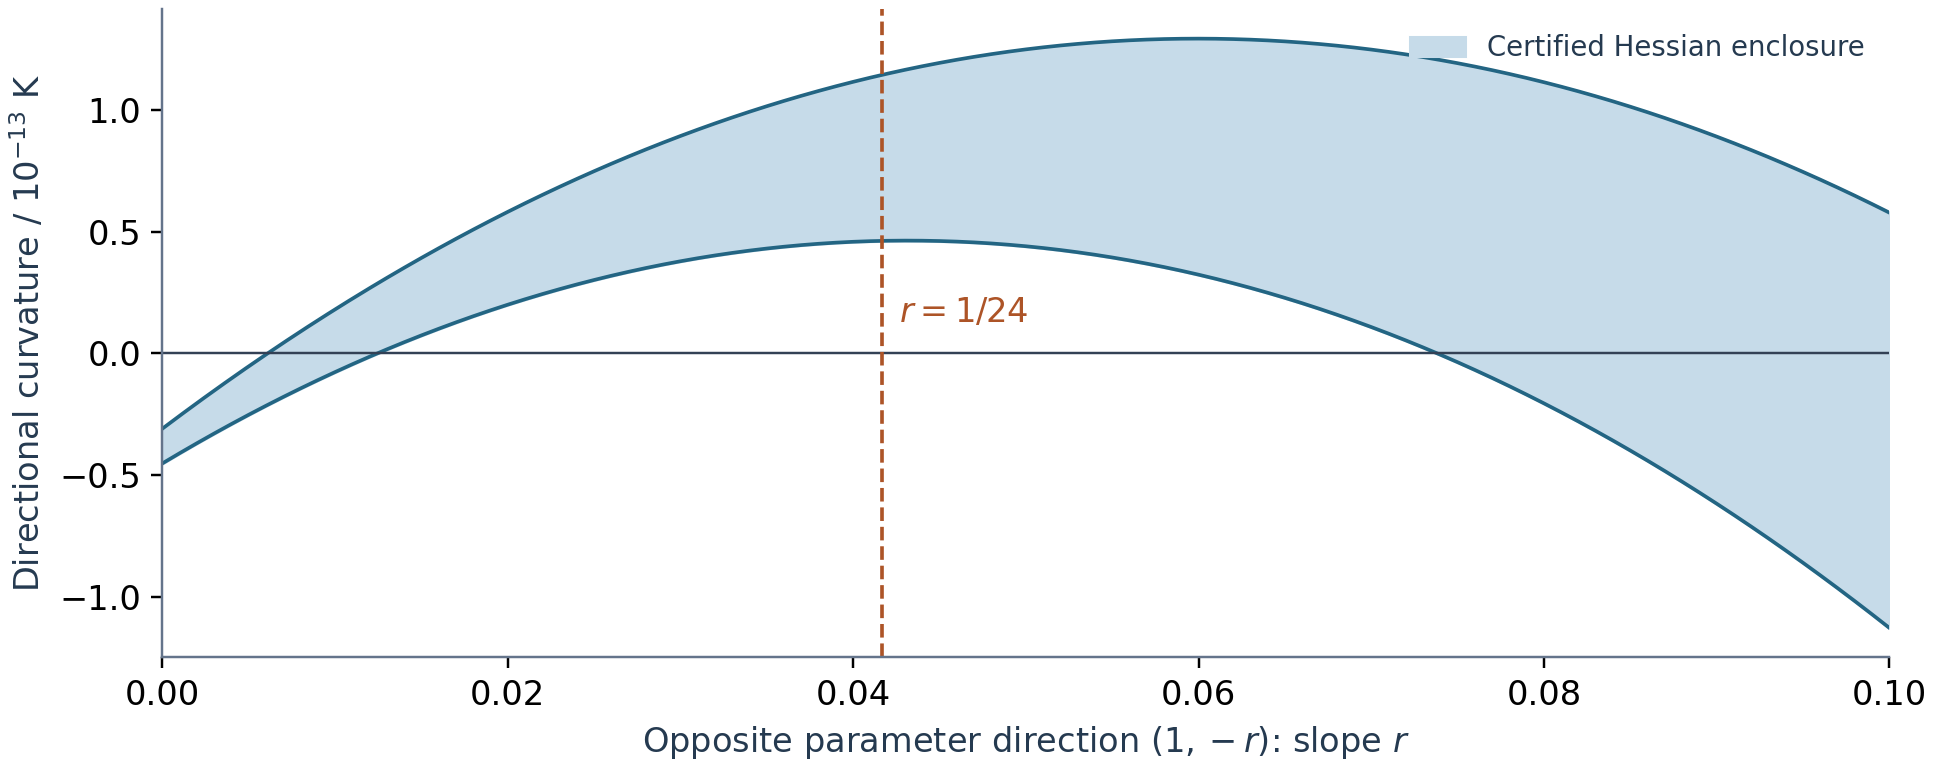
\includegraphics[width=0.95\textwidth]{figures/hessian_directions.png}
\caption{방향 $(1,-r)$의 곡률 포함. 원 유리수 포함의 decimal 표시를 이용한 시각화다.
밴드는 확률적 오차 막대가 아니라 허용 Hessian의 포함이며,
$r=1/24$의 엄격한 양성은 별도의 정확한 유리수 계산으로 판정했다.}
\end{figure}

\section{원 residual에서 순수 곡률까지}
\subsection{보통 2차 도함수와 implicit 방정식}
$\theta\in\{\lambda,b\}$에 대해
$p_k=g_{k,\theta}$, $K_k=g_{k,\theta\theta}$라 쓴다.
$K_k$는 Taylor 계수의 두 배인 보통 2차 도함수다.
고정 incoming의 단계 residual $H_k(g_k,\theta)=0$을 두 번 미분하면
\[
J_kp_k+H_{k,\theta}=0,\qquad
\boxed{J_kK_k=-H_{k,gg}[p_k,p_k]-2H_{k,g\theta}p_k-H_{k,\theta\theta}},
\quad J_k=H_{k,g}.
\tag{19.1}
\]
$C^2$ Hessian의 대칭성이 두 교차항의 계수 2를 준다.
같은 Jacobian으로 두 번째 tangent를 푸는 일반 구조는
Safiran--Lotz--Naumann의 Theorem 4.3과 일치한다 \cite{SLN15}.
본 계산의 root branch와 역행렬 포함은 원 인증에 결박했다.

원 gas source와 HH 방향은
\[
B_k(g,\lambda)=F_k^{np}(g)+\lambda q_k(g)\nu_H-2H_kw e_w,
\qquad \nu_H=(1,0,0,-\chi_H)^T.
\tag{19.2}
\]
첫 half와 Full의 incoming은
$Q_1=RZ_0+bJ_\gamma$, $Q_F=R_FZ_0+2bJ_\gamma$다.
고정 gas에서 각 residual이 $\lambda,b$에 affine이므로
$H_{k,\theta\theta}=0$이다.
원 \texttt{SOURCE\_BOX}의 \texttt{G\_gg,G\_g\_lambda,G\_g\_b}에는
이미 residual 부호와 시간 인수가 들어 있다. 이 export에는 (19.1)을 직접 적용한다.
source Hessian을 분해할 때에만 식 (19.2)의 $h$ 또는 $2h$를 붙인다.

\subsection{survival과 실제 carry}
활성 photon slot $j$에서 $a_{kj}=cn_k\sigma_j$,
$A_k=(1+ha_k(1-x_k))^{-1}$, $L_k=1-A_k$다.
고정 $a_k$에 대한 두 미분은
\[
A_{k,\theta}=ha_kA_k^2p_{k,x},\qquad
\boxed{A_{k,\theta\theta}
=ha_kA_k^2K_{k,x}+2(ha_k)^2A_k^3p_{k,x}^2}.
\tag{19.3}
\]
Full에서는 $ha_k$를 $2ha_2$로 바꾼다.
$\delta_b=\partial_\theta b$를 쓰면
\[
\begin{aligned}
Z_1&=A_1Q_1,& Q_2&=RZ_1+bJ_\gamma,\\
Z_{1,\theta\theta}&=A_{1,\theta\theta}Q_1
2\delta_b A_{1,\theta}J_\gamma,&
Q_{2,\theta\theta}&=RZ_{1,\theta\theta}.
\end{aligned}
\tag{19.4}
\]
첫 단계 gas의 $K_1$과 광자의 $Q_{2,\theta\theta}$를 순서대로 carry한다.
특히 $b=0$에서도 $2A_{1,b}J_\gamma$는 일반적으로 남는다.
생성 진폭의 값과 그 미분은 구별되기 때문이다.

guard는 국소적으로 $A=1,L=0$이어서 이 두 함수의 도함수는 0이다.
그러나 $(RZ_{1,\theta\theta})_{\rm guard}$는
활성 photon의 수송이 guard에 도달하면 남는다.
따라서 incoming/outgoing guard의 순수 응답도 저장했다.

\subsection{carried 둘째 half의 선형 방정식}
둘째 gas 방정식과 Jacobian은
\[
g_2-g_1=hB_2(g_2,\lambda)+V_{\rm ph}L_2(g_2)Q_2,\qquad
J_2=I-hB_{2,g}-V_{\rm ph}(L_{2,g}Q_2).
\]
$p=p_2$, $\delta_\lambda=\partial_\theta\lambda$라 놓으면
\[
\boxed{\begin{aligned}
J_2K_2={}&K_1+hB_{2,gg}[p,p]
2h\delta_\lambda Dq_2[p]\nu_H\\
&+V_{\rm ph}\{L_{2,gg}[p,p]Q_2
+2L_{2,g}[p]Q_{2,\theta}+L_2Q_{2,\theta\theta}\}.
\end{aligned}}
\tag{19.5}
\]
실제 photon 흡수의 순수 도함수에는
$L_{2,g}[K_2]Q_2$도 있다.
이 선형 항은 (19.5)의 $J_2$에 배치하고, $K_2$를 구한 뒤 실제 photon jet를 복원한다.
Full의 birth 항은 product-rule 계수 2와 $Q_{F,b}=2J_\gamma$가 만나
source 표현에서 계수 4를 갖는다.

단계 차이 $s=g_2-g_1$에 대해서도
\[
s_{\theta\theta}
=h\{B_{2,g}K_2+B_{2,gg}[p,p]
+2\delta_\lambda Dq_2[p]\nu_H\}+V_{\rm ph}P_{2,\theta\theta}
\tag{19.6}
\]
를 계산하여 $[K_2]-[K_1]$와 교차한다.

\subsection{같은 Full Jacobian에서 endpoint 차이 보존}
Full residual을 $H(g;\lambda,b)$,
$r=H(g_2;\lambda,b)$,
$d=g_2-g_F$,
$d_\theta=p-p_F$,
$K_d=K_2-K_F$라 쓴다.
모든 endpoint 전달은 $J_F=H_g(g_F)$를 사용한다.
직접식은
\[
J_FK_d=J_FK_2+H_{gg}(g_F)[p_F,p_F]+2H_{g\theta}(g_F)p_F.
\tag{19.7}
\]
$J_y=H_g(g_2)$,
$\Delta H_{gg}=H_{gg}(g_2)-H_{gg}(g_F)$,
$\Delta H_{g\theta}=H_{g\theta}(g_2)-H_{g\theta}(g_F)$라 두자.
대칭 bilinear map에 대한 정확한 항등식
\[
H_{gg}(g_F)[p,p]-H_{gg}(g_F)[p_F,p_F]
=2H_{gg}(g_F)[d_\theta,p-d_\theta/2]
\]
으로 같은 forcing을 다시 쓰면
\[
\boxed{\begin{aligned}
J_FK_d={}&r_{\theta\theta}-(J_y-J_F)K_2-\Delta H_{gg}[p,p]\\
&-2H_{gg}(g_F)[d_\theta,p-d_\theta/2]\\
&-2\Delta H_{g\theta}p-2H_{g\theta}(g_F)d_\theta.
\end{aligned}}
\tag{19.8}
\]
이 식은 큰 endpoint 값을 각각 뺄 때 생기는 포함폭을,
원 작은 차이의 포함으로 직접 제어한다.

$J_y-J_F$와 HH gradient 차이에는 기존 Hessian의 선분 적분을 쓴다.
일반 source의 $\Delta H_{gg}$는 두 평가점의 원 signed Hessian 범위의 차로 포함한다.
HI rational 항은 명시적 분모차를 $d_x$로 인수 분해한다.
따라서 모든 유도와 적용에서 source의 최고 도함수는 2차로 유지된다.

\subsection{gas stage 잔차의 원식 기반 분해}
두 stage 방정식을 더하여
\[
r=h\{B_1(g_1)-B_2(g_2)\}+V_{\rm ph}p_{\rm ph}
\]
를 얻는다. gas 부분의 순수 미분은
\[
\begin{aligned}
r_{g,\theta\theta}=h\{&
B_{1,g}K_1-B_{2,g}K_2
+B_{1,gg}[p_1,p_1]-B_{2,gg}[p,p]\\
&+2\delta_\lambda(Dq_1[p_1]-Dq_2[p])\nu_H\}.
\end{aligned}
\tag{19.9}
\]
$\delta B_t=B_1-B_2$, $\delta q_t=q_1-q_2$라 놓으면
\[
\begin{aligned}
B_{1,g}K_1-B_{2,g}K_2
={}&D\delta B_t(g_1)[K_1]-B_{2,g}(g_2)s_{\theta\theta}\\
&-\int_0^1B_{2,gg}(g_1+ts)[s,K_1]\,\dd t,\\
B_{1,gg}[p_1,p_1]-B_{2,gg}[p,p]
={}&\Delta B_{gg}[p_1,p_1]
-2B_{2,gg}[s_\theta,(p+p_1)/2],\\
Dq_1[p_1]-Dq_2[p]
={}&D\delta q_t(g_1)[p_1]-Dq_2(g_2)[s_\theta]\\
&-\int_0^1D^2q_2(g_1+ts)[s,p_1]\,\dd t.
\end{aligned}
\tag{19.10}
\]
PHYS17의 원 density/temperature pullback에 방향 $K_1$ 또는 $p_1$을 대입했다.
gradient를 새 방향에 평가하는 계산이며, source Hessian 위의 새 미분을 요구하지 않는다.

\subsection{일곱 photon sector와 순서 있는 미분}
$A=A_2$, $L=I-A$, $\tau=ha_2(1-x_2)$,
$A_F=(I+2\tau)^{-1}$,
$L_F=I-A_F$,
$\mathcal C_1=\tau A^2A_F$,
$\mathcal C_2=\tau^2A^2A_F$로 두자.
이 $\mathcal C_i$는 역행렬 preconditioner $C$와 별개다.
원 순서 있는 photon 잔차는
\[
\begin{aligned}
p_{\rm ph}={}&-(I-LR)(A_1-A)Q_1+L[R,A]Q_1
+L(I-R)RZ_0\\
&+\mathcal C_2R^2Z_0+L_F(R^2-R_F)Z_0\\
&+bLA(R-I)J_\gamma-b\mathcal C_1J_\gamma.
\end{aligned}
\tag{19.11}
\]
$R$와 diagonal survival의 순서를 바꾸지 않는다.
$D_A=(A_1-A)Q_1$,
$K_R=[R,A]Q_1$,
$Z_R=(I-R)RZ_0$,
$J_R=(R-I)J_\gamma$라고 쓰고 prime을 $\theta$ 미분으로 쓰면,
일곱 항의 순수 응답은
\[
\begin{aligned}
p_{\rm opacity}''&=-D_A''+L''RD_A+2L'RD_A'+LRD_A'',\\
p_{\rm comm}''&=L''K_R+2L'K_R'+LK_R'',\\
p_{\rm stockR}''&=L''Z_R,\qquad
p_{\rm stockBE}''=\mathcal C_2''R^2Z_0,\\
p_{\rm remap}''&=L_F''(R^2-R_F)Z_0,\\
p_{\rm birthR}''&=\{b(LA)''+2\delta_b(LA)'\}J_R,\\
p_{\rm birthBE}''&=-\{b\mathcal C_1''+2\delta_b\mathcal C_1'\}J_\gamma.
\end{aligned}
\tag{19.12}
\]
각 matrix product의 보통 순수 도함수는
$(XY)''=X''Y+2X'Y'+XY''$다.
opacity 차이는
\[
A_1-A=\zeta A_1A,\quad
\zeta=h\{c\sigma(n_2-n_1)(1-x_2)-a_1s_x\},
\]
\[
\zeta''=-h\{c\sigma(n_2-n_1)K_{2,x}+a_1s_{\theta\theta,x}\}
\tag{19.13}
\]
로 인수 분해한 뒤 미분했다.
이렇게 얻은 일곱 sector와 직접 흡수 차이의 포함을 같은 35개 slot에서 확인했다.

$\Delta\widehat Z=Z_2-A_F(g_2)Q_F$와 원 number·energy row를 쓰면
\[
\mathbf1^Tp_{\rm ph}''=-n_\gamma\Delta\widehat Z'',\qquad
E^Tp_{\rm ph}''=(1-\rho)E^TP_1''-u_\gamma\Delta\widehat Z''
\tag{19.14}
\]
가 성립한다. $\rho$는 원 redshift 비다.
직접 birth energy 항은 $b$에 선형이므로 이 순수 미분에서는 0이다.
원 ledger의 두 guard를 유지한 것이 (19.14)의 의미다.

\subsection{검증된 inverse의 재사용}
각 stage의 고정 $C$, 비음수 $B$, 양의 scale $S$에 대해
\[
|I-CJ|\le B,\qquad \|S^{-1}BS\|_\infty\le q<1
\tag{19.15}
\]
를 원 입력과 대조했다.
$Jv=f$에서 $v=Cf+(I-CJ)v$이고
$(I-B)^{-1}=\sum_{k\ge0}B^k\ge0$이므로
\[
m=(I-B)^{-1}\operatorname{mag}([Cf]),\qquad
\boxed{v\in[Cf]+[-Bm,Bm]}.
\tag{19.16}
\]
이는 family의 모든 허용 Jacobian과 RHS를 포함한다.
interval family 전체의 가역성·해 포함이라는 양화는 Rump의
검증된 선형계 구성과 일치한다 \cite{R99}.
현재 수치는 원 고정 행렬과 유리수 majorant로 직접 계산했다.
signed $[I-CJ]$를 남겨 세 번의 유한 fixed-point 교차를 적용했다.

첫 half의 결박은
\[
C=I,\qquad S=\operatorname{diag}(1,1,1,27/2),\qquad q<0.0005396
\]
이다. Full은 원 $q=0.00011736830563768177$의 exact64 leaf를 사용한다.
둘째 half의 refined contraction은 $q<0.0005045844357588$이다.
endpoint $K_d$의 모든 분해와 기여에는 Full의 동일한 $C,B,S,J_F$를 썼다.
직접·상관·별도 endpoint 차이는 동일 exact quantity의 포함이므로 교차가 유효하다.

\section{유한 온도 quotient와 인증된 재구성}
\subsection{온도 도함수를 같은 endpoint 식으로 읽기}
원 온도 정의는
\[
\ell_e=(1,f,2f,0),\quad \Pi(g)=1+f+\ell_eg,\quad
C_T=\frac{2\epsilon_{\rm eV}}{3k_B},\quad
T(g)=\frac{C_Tw}{\Pi(g)}.
\tag{19.17}
\]
정확한 항등식 $T\Pi=C_Tw$를 미분하면
\[
T_{2,\theta\theta}
=\frac{C_TK_{2,w}-T_2\ell_eK_2-2T_{2,\theta}\ell_ep}{\Pi_2}.
\tag{19.18}
\]
$d_e=\ell_ed$, $d_{e,\theta}=\ell_ed_\theta$,
$\Pi_{F,\theta}=\ell_ep_F$,
$n_F=C_Te_w^T-T_F\ell_e$라 놓는다.
두 온도 차이의 유한 quotient를 두 번 미분하고
같은 $K_d$에 묶으면
\[
\boxed{
F_{\theta\theta}
=\frac{
n_FK_d
-T_{2,\theta\theta}d_e
-2T_{2,\theta}d_{e,\theta}
-2F_\theta\Pi_{F,\theta}
-F\ell_eK_2}{\Pi_F}.}
\tag{19.19}
\]
모든 분모는 원 positive enclosure를 사용한다.
gas의 각 sector $r_j$를 $(n_F/\Pi_F)J_F^{-1}r_j$로 읽고,
나머지 네 항을 온도 geometry로 보존했다.
이 읽기와 직접 $T_{2,\theta\theta}-T_{F,\theta\theta}$의 포함도 교차했다.
이 과정에서 HH 방향의 $-\chi_H$와 전자수에 따른 $\Pi$ 변화가 모두 남는다.

\subsection{같은 계열의 네 corner와 bilinear 항}
$F_{ij}=F(i,j)$로 쓰자. 네 값은 같은 고정 $\alpha$의
같은 COMMON 계열에서 평가된 함수값이다.
\[
\begin{gathered}
a_\lambda=F_{10}-F_{00},\qquad a_b=F_{01}-F_{00},\\
\mathcal I=F_{11}-F_{10}-F_{01}+F_{00},\\
\mathcal LF=F_{00}+a_\lambda\lambda+a_bb+\mathcal I\lambda b.
\end{gathered}
\tag{19.20}
\]
기본정리에 따라 $a_\lambda,a_b$는 축 첫 도함수의 적분이고,
$\mathcal I=\int_0^1\int_0^1F_{\lambda b}(u,v)\,\dd u\,\dd v$다.
따라서 원 포함만으로 이 계수들의 안전한 범위를 얻는다.
점별 $F_{\lambda b}$와 적분값 $\mathcal I$는 서로 다른 양이다.
현재 PHYS18에서는 같은 구간으로 포함되며, 최종 readout에서는 각각의 원 필드에 따로 결박했다.

\subsection{signed Peano kernel의 직접 증명}
1차원 endpoint 선형 보간 $I_xf=(1-x)f(0)+xf(1)$에 대해
두 번의 부분적분으로
\[
f(x)-I_xf(x)=\int_0^1K_x(t)f''(t)\,\dd t,\qquad
K_x(t)=
\begin{cases}
-t(1-x),&t\le x,\\
-x(1-t),&t\ge x
\end{cases}
\tag{19.21}
\]
를 얻는다.
$K_x\le0$이고 $\int_0^1K_x(t)\,\dd t=-x(1-x)/2$다.
두 축 interpolation 연산자에
$I-I_\lambda I_b=(I-I_\lambda)+I_\lambda(I-I_b)$를 쓰자.
$I_\lambda$의 endpoint weights는 비음수이고 합이 1이므로,
전체 사각형에서 $F_{\lambda\lambda}\in[A]$, $F_{bb}\in[D]$이면
\[
\boxed{
F-\mathcal LF\in
-\frac{\lambda(1-\lambda)}2[A]
-\frac{b(1-b)}2[D].}
\tag{19.22}
\]
이는 tensor-product 보간의 pure-derivative 상계 \cite{MR09}를
현재 부호 정보까지 살린 직접 구성이다.
$C^2$ 정칙성으로 충분하며, 혼합 4차 미분이 필요하지 않다.

$M_A=\max_{a\in[A]}|a|$, $M_D=\max_{d\in[D]}|d|$라 두면
\[
\boxed{\|F-\mathcal LF\|_\infty\le\frac{M_A+M_D}{8}
\le6.145761081776\times10^{-12}\ {\rm K}.}
\tag{19.23}
\]
두 순수 곡률의 엄격한 음성 때문에
$F-\mathcal LF\ge0$이며,
corner를 제외한 경계점과 모든 내부점에서는 양수다.
중심에서는 더 구체적으로
\[
F(1/2,1/2)-\mathcal LF(1/2,1/2)
\in[5.567183547133,6.145761081776]10^{-12}\ {\rm K}.
\tag{19.24}
\]

\subsection{순수 곡률 중심으로 보정한 유한 다항식}
$c_A,c_D$를 정확한 구간 중심,
$r_A,r_D$를 정확한 반폭으로 두고
\[
\mathcal QF=\mathcal LF
-\frac{c_A}2\lambda(1-\lambda)
-\frac{c_D}2b(1-b)
\tag{19.25}
\]
를 정의한다.
이 함수의 순수 두 도함수는 각각 $c_A,c_D$이며 corner는 그대로다.
식 (19.22)를 $F-\mathcal QF$에 적용하면
\[
\boxed{\|F-\mathcal QF\|_\infty\le\frac{r_A+r_D}{8}
\le2.892887673208\times10^{-13}\ {\rm K}.}
\tag{19.26}
\]
상계는 $21.24438200174$배 이상 줄어든다.
전달하기 쉬운 유한 decimal 계수
\[
c_A^{\rm dec}=-3.797385260416\times10^{-14}\ {\rm K},\qquad
c_D^{\rm dec}=-4.681380466304\times10^{-11}\ {\rm K}
\tag{19.27}
\]
를 정확한 유리수로 사용하면 중심 반올림의 거리도 반폭에 더해야 한다.
이를 반영한 실제 사용 가능 상계는
$2.892887673216\times10^{-13}\ {\rm K}$다.
보고서의 $2.893\times10^{-13}\ {\rm K}$라는 짧은 표기는 이 값을 바깥으로 반올림한 것이다.

\begin{figure}[H]\centering
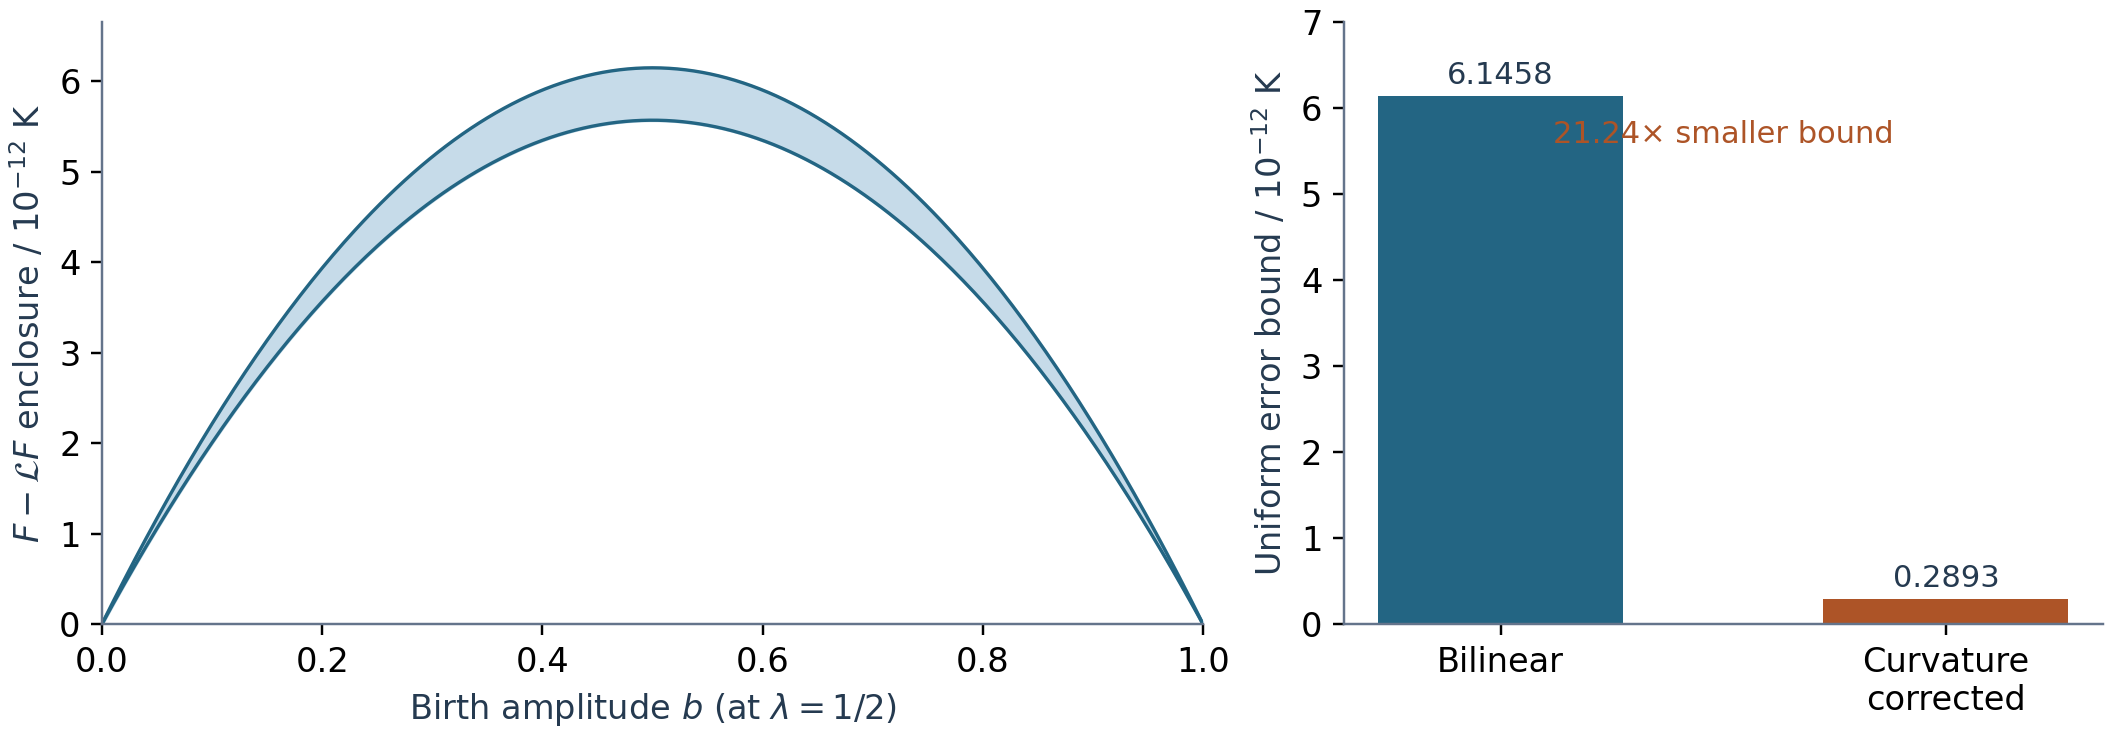
\includegraphics[width=0.98\textwidth]{figures/interpolation_error.png}
\caption{왼쪽: $\lambda=1/2$에서 인증된 bilinear 재구성의 signed error 포함.
오른쪽: 형상 재구성의 두 균일 상계 비교.
이는 계산된 inclusion 공식의 시각화이며, 물리 함수의 표본 시뮬레이션이 아니다.}
\end{figure}

\subsection{계수 해상도를 포함한 중심값 모델}
식 (19.23)--(19.26)은 실제 동일 계열 corner 계수를 유지한 형상 오차다.
수치 다항식을 얻으려면 $F_{00},a_\lambda,a_b,\mathcal I$도
구간 중심값으로 바꾸므로 그 계수 불확실성이 추가된다.
이 해상도를 함께 제시해야 유한 surrogate의 정확한 의미가 드러난다.

원 전체 온도 결함 포함을 $G$라 하자.
네 corner 모두 $G$에 속하므로
\[
[F_{00}]\leftarrow G\cap(G-[a_\lambda])\cap(G-[a_b])
\cap(G-[a_\lambda]-[a_b]-[\mathcal I])
\tag{19.28}
\]
로 안전하게 조일 수 있다.
원 $G=[-0.001585967387182,-0.001210819969055]\ {\rm K}$에서
다음 구간을 얻었다.
\begin{table}[H]\centering\small
\caption{실제 계수를 담는 외향 포함. 네 계수의 같은-family 관계는 유지한다.}
\begin{tabular}{ll}
\toprule
계수 & Kelvin 단위 포함\\
\midrule
$F_{00}$ & $[-0.001585959249676,-0.001278583452911]$\\
$a_\lambda$ & $[-1.009599125635,-0.8137506081166]10^{-8}$\\
$a_b$ & $[6.776348385589,7.185335549648]10^{-5}$\\
$\mathcal I$ & $[-2.668505746423,-2.118796636045]10^{-12}$\\
\bottomrule
\end{tabular}
\end{table}
각 중심을 $m_0,m_\lambda,m_b,m_I$, 반폭을 $r_0,r_\lambda,r_b,r_I$라 쓰고,
(19.27)을 사용한 수치 모델을
\[
P=m_0+m_\lambda\lambda+m_bb+m_I\lambda b
-\frac{c_A^{\rm dec}}2\lambda(1-\lambda)
-\frac{c_D^{\rm dec}}2b(1-b)
\]
로 정의한다.
$\widetilde r_A=\max_{a\in[A]}|a-c_A^{\rm dec}|$와
$\widetilde r_D$를 쓰면 점별 오차는
\[
\begin{aligned}
|F-P|\le{}&
r_0+r_\lambda\lambda+r_bb+r_I\lambda b\\
&+\frac{\widetilde r_A}{2}\lambda(1-\lambda)
+\frac{\widetilde r_D}{2}b(1-b).
\end{aligned}
\tag{19.29}
\]
따라서 이 전체 중심값 모델의 보수적인 균일 오차 상계는
\[
\boxed{\|F-P\|_\infty\le0.0001557338140092\ {\rm K}.}
\tag{19.30}
\]
모든 중심과 반폭은 정확한 유리수로 결과 JSON에 저장했다.
계수의 포함폭은 현재 family 정보의 해상도이며 실제 오차의 관측값은 아니다.
이를 줄이려면 특정한 $\alpha$와 실제 소비 상태를 결박한 추가 정보가 필요하다.
이번의 매우 작은 곡률 보정 오차는 그 다음 판단에 쓸 수 있는 재구성 부분을 닫아 준다.

\section{실제 계산과 독립 검증}
\subsection{동결 입력, 실행과 정밀도}
PHYS18의 최종 commit과 연구 묶음을 기준으로 시작했다.
채택된 곡률 계약의 23개 입력은 경로·바이트 수·SHA-256이 모두 일치했다.
PHYS15--18의 기존 source box, root·carry·inverse 및 response 포함을
그 원본 의미와 identity에 결박해 재사용했다.

\texttt{src/curvature\_application.py}는 정확한 Fraction 연산에
256-bit dyadic 외향 반올림을 결합한다.
순수 jet의 곱과 역수에는 보통 2차 도함수 계수를 사용했다.
첫 half·Full·carried 둘째 half,
직접·상관 endpoint forcing,
35개 photon slot, 일곱 sector, number·energy ledger와 온도 quotient를
한 번의 실제 계산에서 출력했다.
실행 전에 명령·code hash·환경·시간 예산을 기록했다.

\begin{table}[H]\centering\small
\caption{완료한 계산의 범위와 실제 비용.}
\begin{tabularx}{\textwidth}{lXl}
\toprule
실행 & 계산 범위 & 경과\\
\midrule
application run01 & 동결 원 입력의 순수 곡률 포함 생성 & wrapper 1.569 s\\
application 내부 & 동일 실행의 실제 계산 구간 & 1.407 s\\
geometry readout02 & 정확한 유리수 Hessian·보간·계수 예산 & 0.049 s\\
독립 Fraction run03 & 별도 산술의 실제 포함·readout 검증 & wrapper 1.870 s\\
Wolfram run01 & 실제 xAct와 symbolic 순수 항등식 & API 13.222 s\\
Wolfram 내부 & 같은 요청의 kernel 대수 계산 & 2.000 s\\
Wolfram run02 & decimal 입력을 exact rational로 한 Hessian 방향 검산 & API 6.088 s\\
\bottomrule
\end{tabularx}
\end{table}
Python 환경은 3.12.14, Linux x86-64다.
main wrapper의 최대 RSS는 55,992 KiB, 계산 내부 기록은 47,544 KiB다.
geometry의 readout01은 계산 결과를 먼저 생성했고,
readout02에서는 점별 혼합 미분과 corner 적분 계수의 입력 필드를 분리했다.
두 SUMMARY의 정확한 endpoint는 전부 같았다.
원 실행과 두 readout 기록을 각각 보존했다.

새 atomic source 호출, reaction fit, nonlinear root solve 및 history replay의 횟수는
각각 0이다. 이번 실행의 대상은 이미 검증된 원 입력에서 새 순수 도함수와
유한 응답 포함을 계산하는 것이었다.

\subsection{Wolfram과 xAct의 실제 사용}
연결된 Wolfram 15.0.1 Linux kernel에서 공식
xAct 1.3.0 archive를 내려받아 hash를 대조하고
xTensor 1.3.0·xPerm 1.2.4를 실제 로드했다.
tensor canonicalization은 \texttt{\$xpermQ=False}인 Wolfram Language group backend다.
패키지 초기화의 external xPerm 메시지와 실제 선택한 backend를 구분해 기록했다.

첫 요청의 6개 tensor 항등식, 13개 scalar 항등식,
14개 matrix component가 모두 literal 0을 반환했고,
Peano kernel의 부호·질량·weight에 관한 4개 부등식은 모두 True였다.
검산은 implicit 계수 2,
carried $Q_2''$,
Full birth 계수,
대칭 Hessian 차이,
원 순서의 일곱 photon sector,
유한 온도 quotient와 보간 kernel을 포함했다.
matrix sector 검산에는 임의의 비가환 2-slot remap을 사용했다.
35개 실제 photon slot의 수치 포함은 별도의 application과 독립 심사에서 확인한다.

첫 요청에는 임시 symbol 이름에 대한
\texttt{Symbol::undefined2} 진단이 있었다.
제출된 Module의 local 이름과 대입을 확인했고,
지정한 residual은 모두 평가된 0이었다.
원 경고·초기화 메시지·request·response를 보존했다.
두 번째 Hessian 요청은 경고 없이 완료됐으며,
별도의 두 방향 수축 항등식도 정확히 0이었다.
decimal 표시를 exact rational로 사용한 별도 포함은
main의 원 유리수 포함보다 약간 넓지만 동일한 엄격한 부호를 준다.

\subsection{독립 심사와 채택}
독립 원식 유도는 $C^2$ 계약에서 C3--C20의 부호·계수를 확인했다.
별도 Fraction interval class, 이항계수 pure jet, Gaussian elimination으로
실제 producer의 산술을 import하지 않고 포함을 재계산했다.
최종 run03에서 362개 검사,
265개 비교 묶음의 2,057개 스칼라 포함,
3,174개 외향 decimal 표시,
23개 계약 입력이 모두 통과했다.
같은 Full inverse, 35개 carried photon slot과 일곱 sector,
endpoint·온도 quotient 및 유한 응답을 독립적으로 확인했다.
number·energy ledger의 별도 수치 잔차는 모두 0을 포함했으며,
정확한 보존식의 증명은 원식 유도에 연결했다.

독립 검산 wrapper의 경과는 1.870 s, 최대 RSS는 52,448 KiB다.
앞선 두 짧은 시도는 검사기의 정규화 비교와 변수 shadowing을 고친 뒤 종료했고,
세 실행의 snapshot·실패 기록을 모두 보존했다.
수정 대상은 독립 검사기였으며 scientific producer와 원 입력·결과는 그대로다.
최종 독립 판정은 \texttt{PASS\_SCOPED}다.
Root는 검토된 source·result·readout hash를 다시 대조한 뒤,
현재 고정 계열에서 \texttt{PROMOTE\_SCOPED}로 채택했다.

원 유도 문서는
\texttt{theory/PURE\_CURVATURE\_INDEPENDENT\_DERIVATION\_KO.md}에
보다 세부적인 C3--C20 대응과 모든 부호·극한 검토를 보존했다.
HH source가 항등적으로 0인 경우의 $\lambda$ 응답,
birth가 0인 경우의 $b$ 응답,
투명 opacity 극한,
같은 endpoint 계열에서의 결함 소멸,
bilinear 함수와 corner에서의 정확한 재현을 원식으로 점검했다.
이 극한들은 실제 source의 추가 실행으로 보고하지 않았다.

\subsection{문헌 대조가 지지하는 부분}
SciSpace의 완전한 질문 1회와 Exa의 두 검색(각 6개 후보)에서
관련 문헌을 조사하고, 세 원전의 실제 해당 본문을 대조했다.
Exa에서 RWTH PDF의 본문 회수가 비어 나온 한 사례는
별도 web 원문 열기로 확인을 마쳤다.
상세 요청·후보·접근 상태와 읽은 위치는 문헌 provenance에 있다.

일반 implicit 2차 미분 \cite{SLN15},
검증된 interval inverse의 family 양화 \cite{R99},
순수 편미분만을 사용하는 tensor-product 보간 경계 \cite{MR09}는
기존 수학 구조다.
이번의 구체적인 연구 진전은 원 gas--photon carry,
HH와 birth의 전역 parameter identity,
상관된 endpoint 잔차와 유한 온도 quotient를 결합해
실제 Kelvin 단위의 부호와 오차 포함을 닫은 데 있다.

\section{다음 루프의 물리 질문과 인계}
\subsection{PHYS20: 실제 소비 구간의 HH source 응답}
다음 목표는 실제로 이름과 원 입력을 지정한
rei\_bianchi 소비 구간 하나에서
HH의 절대 열 변화율과 전자 생성률을 구하는 것이다.
첫 행동은 최신 채택 entry에서 해당 구간의 source,
COMMON, 상태와 단위, density/frame, clock,
geometry/tilt, closure와 process owner를 좁게 회수해 결박하는 것이다.
현재 consumer 결박은 이번 루프에서 확인하지 않았으므로
\texttt{unverified}로 인계한다.

원 readout과 해당 소비자의 HH stoichiometry가 채택되면
\[
\dot g_{\rm HH}=\nu_Hq_{\rm HH},\qquad
\dot T_{\rm HH}
=\frac{C_Te_w^T-T\ell_e}{\Pi}\nu_Hq_{\rm HH},\qquad
\dot e_{\rm HH}=\ell_e\nu_Hq_{\rm HH}
\tag{19.31}
\]
를 외향 포함한다.
여기서 $q_{\rm HH}$는 실제 HH 활성 계수까지 포함한 이벤트율이다.
원 FT03/LCS의 $\nu_H=(1,0,0,-\chi_H)^T$가 admitted되면
\[
\boxed{\dot T_{\rm HH}
=-\frac{C_T\chi_H+T}{\Pi}q_{\rm HH},\qquad
\dot e_{\rm HH}=q_{\rm HH},\qquad
(\dot n_e)_{\rm HH}=n_Hq_{\rm HH}.}
\tag{19.32}
\]
단위는 각각 K/s, per H/s, 전자수밀도/s다.
consumer가 $c^{-1}\partial_t$ 정규화를 사용한다면 원 $c$와 clock을 먼저 변환한다.
첫 표에는 같은 상태의 다른 thermal/electron source, signed total,
HH의 절대 기여와 지배 입력을 함께 담는다.
source ownership을 확인해 중복 합산을 피한다.

이 목표는 기존 \texttt{HH\_DOMAIN\_SCREEN}에서
\texttt{HH\_MATERIALITY}로 이어진다.
local source 응답에 필요한 적용성 결박과
PHYS19의 전체 endpoint 인증을 재사용하는 적용성 결박을 각각 그 claim에 맞게 확인한다.
finite interval·matched history는 기존 root/carry 및 RUX11 조건이 결박되면 이어간다.
준비된 인계 계약은 실제 다음 계산을 수행한 결과로 기록하지 않는다.

\subsection{프로젝트 상태와 재현 진입점}
이번 채택은 \texttt{HH\_DEFECT\_PARAMETER\_CURVATURE}의 범위에 한정한다.
기존 RUX 전역 DAG와
\texttt{HH\_STRICT\_NATIVE}, \texttt{HH\_SINGLET}의 독립 질문을 유지한다.
이 두 lane의 원 microscopic/channel/spin 조건은 각자 원 입력에 연결한다.
PHYS20 소비 source 응답과의 완료 의존성을 새로 만들지 않는다.

제공한 묶음에는 보고서 소스·수치 JSON·실행 코드·원 request/response,
입력 identity와 PHYS18 dependency archive, 독립 심사와
다음 consumer 계약이 들어 있다.
최상위 \texttt{REPRODUCE.md}는 이미 완료된 근거를 확인하는 경로와
필요할 때 같은 새 계산만 재현하는 명령을 제시한다.
문서·수치 포함·원 source/root 근거의 상태는
\texttt{review/DECISION.json}과 \texttt{state/RESEARCH\_STATE.json}에 분리해 결박했다.

\begin{thebibliography}{9}
\bibitem{SLN15}
N. Safiran, J. Lotz, U. Naumann,
\emph{Second-order Tangent Solvers for Systems of Parameterized Nonlinear Equations},
Procedia Computer Science 51 (2015), 231--238.
DOI: \href{https://doi.org/10.1016/j.procs.2015.05.232}{10.1016/j.procs.2015.05.232}.
실제 대조: §4.2, Theorem 4.3, Eq. (7), pp.235--236.
\href{https://publications.rwth-aachen.de/record/569704/files/569704.pdf}{저자 기관 PDF}.
\bibitem{R99}
S. M. Rump,
\emph{Verified Solution of Large Linear and Nonlinear Systems},
in Error Control and Adaptivity in Scientific Computing, Kluwer (1999), 279--298.
실제 대조: §3, Lemma 3.1, Theorem 3.2, 저자 PDF pp.4--5.
\href{https://www.tuhh.de/ti3/paper/rump/Ru99d.pdf}{저자 PDF}.
\bibitem{MR09}
B. Mößner, U. Reif,
\emph{Error Bounds for Polynomial Tensor Product Interpolation},
Computing 86 (2009), 185--197.
DOI: \href{https://doi.org/10.1007/s00607-009-0062-7}{10.1007/s00607-009-0062-7}.
실제 대조: 2009-03-18 저자 원고 §3, Theorem 3.1, PDF p.5.
\href{https://www.mathematik.tu-darmstadt.de/media/mathematik/forschung/preprint/preprints/2580.pdf}{저자 원고}.
\bibitem{PHYS18}
WU088\_HH PHYS18, \emph{HH와 birth의 혼합 응답과 유한 상호작용},
2026-10-13. 고정 기준 commit:
\texttt{41fe51d5a40651e8cadbaa52554035b58a92490c}.
\href{https://github.com/cosmosapjw-quantum/WU088_HH/pull/53}{Draft PR 53}.
채택 계약: \texttt{contracts/ADOPTED\_CURVATURE\_CONTRACT.json}.
\end{thebibliography}
\end{document}
